\section{ETFW}
In a virtual machine with the image of \textit{ETFW} you can configure the service via Central Management, on tab \textit{ETFW}.

In the main panel you can access the \textit{Network setup wizard} or access the \textit{Webmin} interface to make changes in any configuration.

The site also has the \textit{Save configuration} option that makes the changes effective. Without this option, any changes made lost after \textit{reboot}.

\begin{figure}[H]
    \begin{center}
    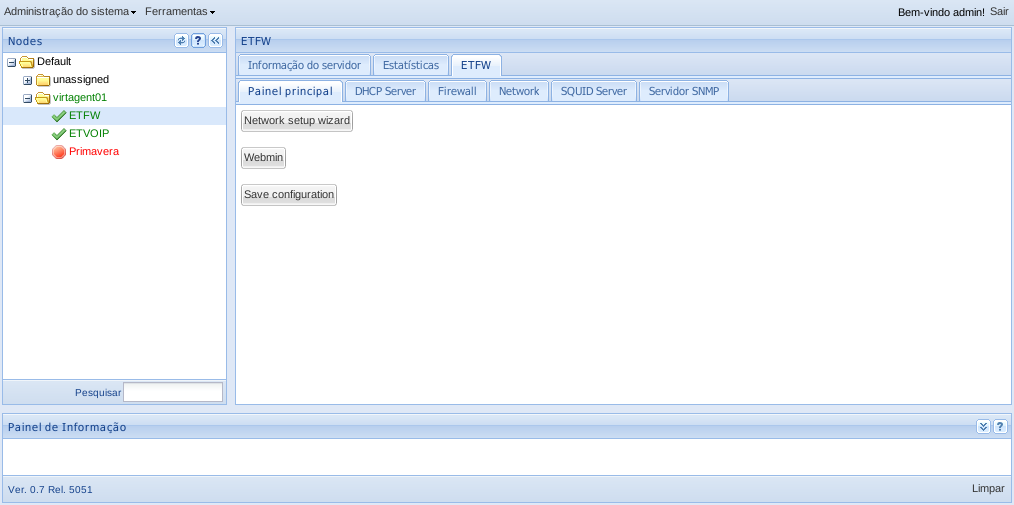
\includegraphics[scale=0.38]{screenshots/etfw/etfwmain.png}
    \caption{Main panel}
    \label{fig:etfwmain}
    \end{center}
\end{figure}

\subsection{Network setup Wizard}

To configure the module \textit{ETFW} quickly and efficiently it's provided a step by step setup wizard.

\begin{figure}[H]
    \begin{center}
    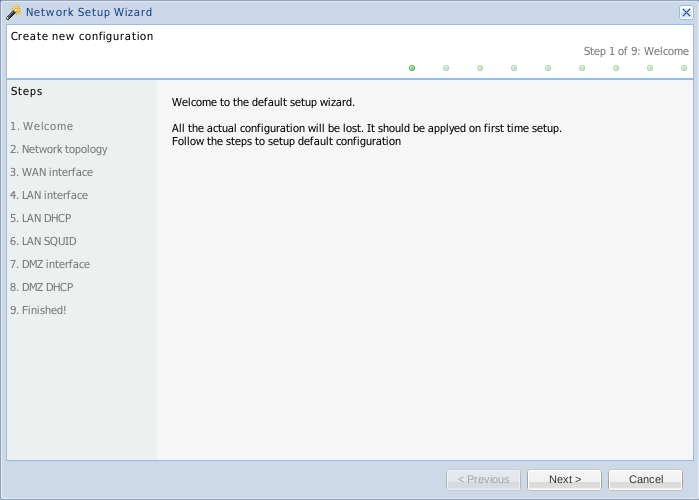
\includegraphics[scale=0.38]{screenshots/etfw/etfw_wizard_01.png}
    \caption{Welcome}
    \label{fig:etfw_wizard_passo1}
    \end{center}
\end{figure}

\begin{figure}[H]
    \begin{center}
    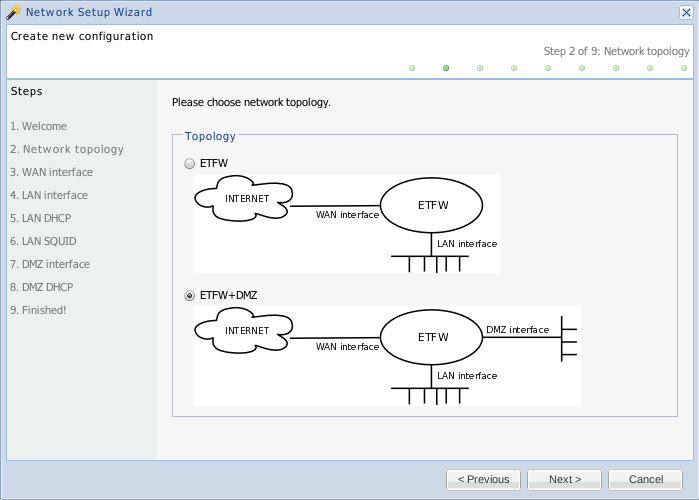
\includegraphics[scale=0.38]{screenshots/etfw/etfw_wizard_02.png}
    \caption{Topology setup}
    \label{fig:etfw_wizard_passo2}
    \end{center}
\end{figure}

\begin{figure}[H]
    \begin{center}
    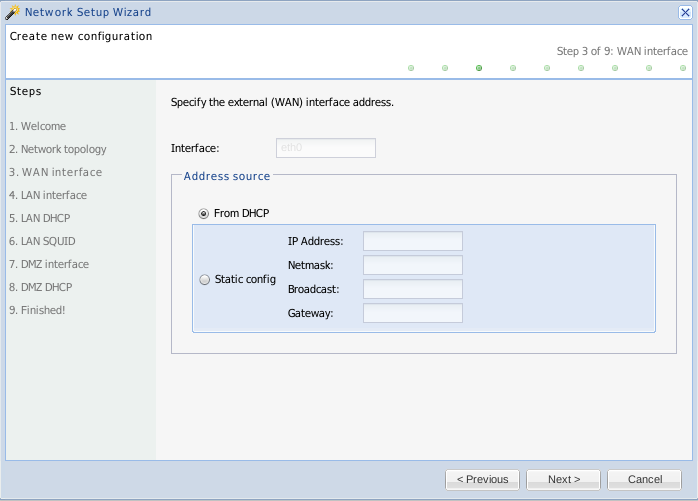
\includegraphics[scale=0.38]{screenshots/etfw/etfw_wizard_03.png}
    \caption{Configuring the WAN interface}
    \label{fig:etfw_wizard_passo3}
    \end{center}
\end{figure}

\begin{figure}[H]
    \begin{center}
    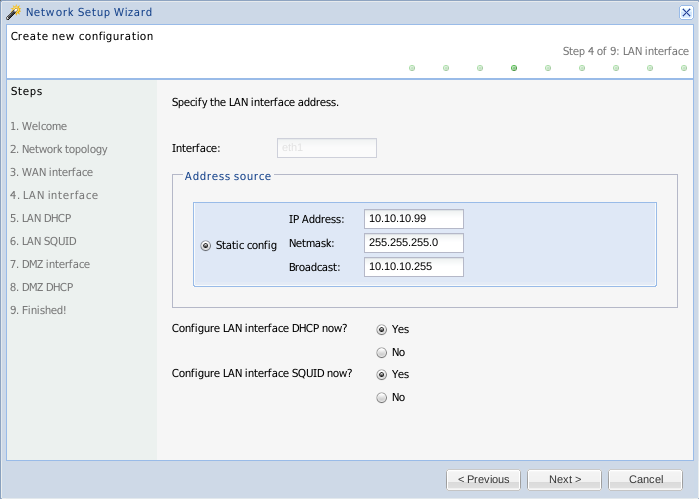
\includegraphics[scale=0.38]{screenshots/etfw/etfw_wizard_04.png}
    \caption{Configuring the LAN interface}
    \label{fig:etfw_wizard_passo4}
    \end{center}
\end{figure}

\begin{figure}[H]
    \begin{center}
    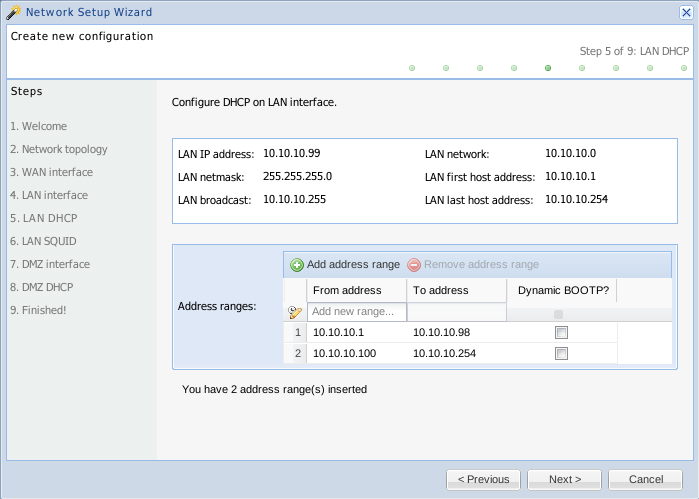
\includegraphics[scale=0.38]{screenshots/etfw/etfw_wizard_05.png}
    \caption{Configuring of the DHCP service for LAN network}
    \label{fig:etfw_wizard_passo5}
    \end{center}
\end{figure}

\begin{figure}[H]
    \begin{center}
    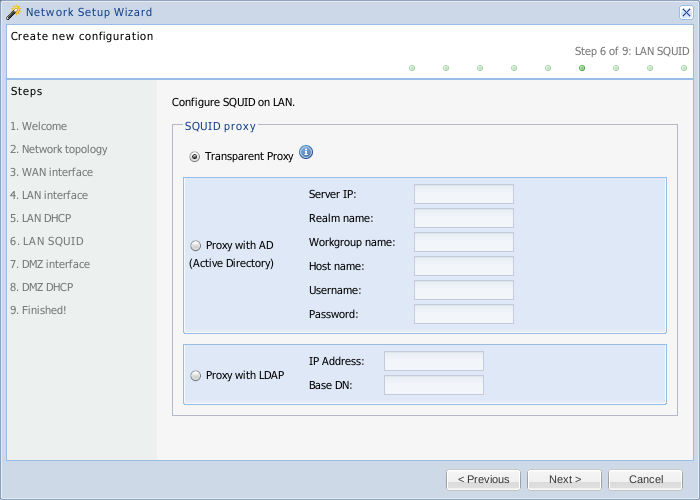
\includegraphics[scale=0.38]{screenshots/etfw/etfw_wizard_06.png}
    \caption{Configuring SQUID proxy}
    \label{fig:etfw_wizard_passo6}
    \end{center}
\end{figure}

\begin{figure}[H]
    \begin{center}
    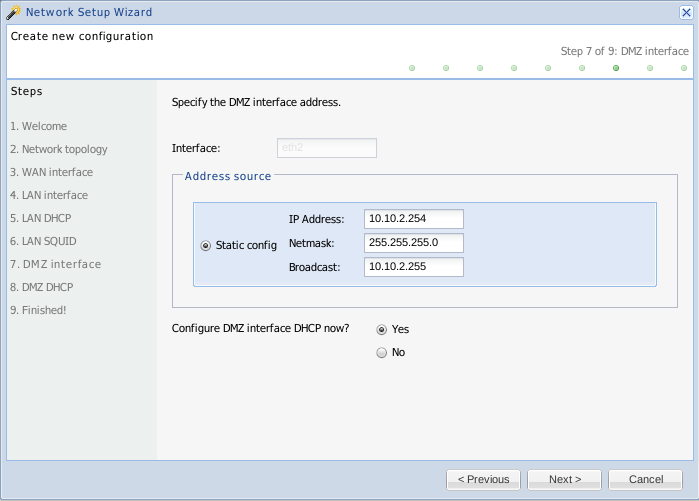
\includegraphics[scale=0.38]{screenshots/etfw/etfw_wizard_07.png}
    \caption{Configuring DMZ interface}
    \label{fig:etfw_wizard_passo7}
    \end{center}
\end{figure}

\begin{figure}[H]
    \begin{center}
    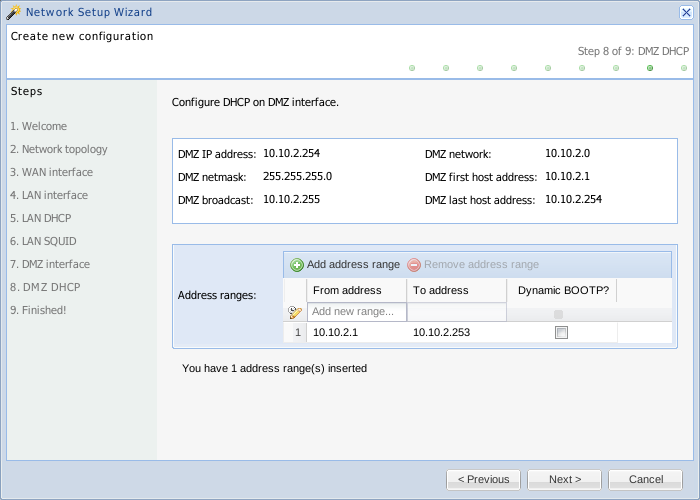
\includegraphics[scale=0.38]{screenshots/etfw/etfw_wizard_08.png}
    \caption{Configuring DHCP service for DMZ network}
    \label{fig:etfw_wizard_passo8}
    \end{center}
\end{figure}

\begin{figure}[H]
    \begin{center}
    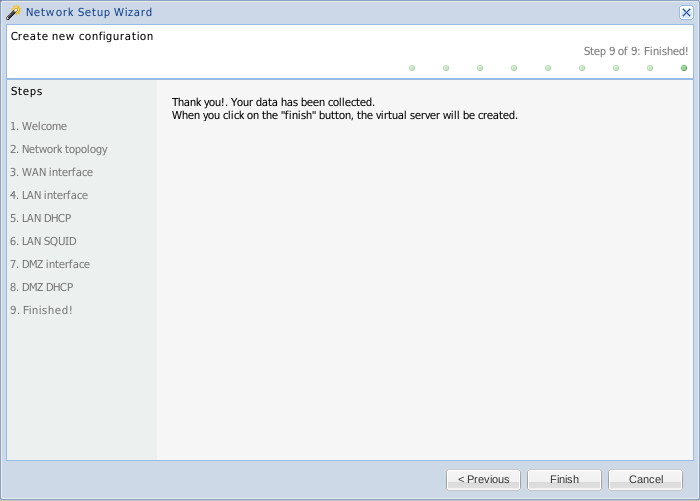
\includegraphics[scale=0.38]{screenshots/etfw/etfw_wizard_09.png}
    \caption{Completion of the configuration}
    \label{fig:etfw_wizard_passo9}
    \end{center}
\end{figure}

\subsection{Network setup - \textit{Network}}
In addition to the wizard configuration process you can change the network configuration manually.
To do this, go to the \textit{network} tab where we have access to the configuration of network interfaces (\textit{Network interfaces}), routing rules (\textit{Routing and gateways}), address configuration (\textit{Host Addresses}) and client \textit{DNS} (\textit{Hostname and DNS client}).

\subsubsection{Network interfaces}
In \textit{Network interfaces} we can see the network interfaces that are configured and which are going to be active at the machine start.

When selecting an interface we can edit the parameters of the interface, such as the IP address, netmask, broadcast, and aliases in virtual interfaces.
To add a new interface, select the add button and fill in the required fields for the interface configuration.

\begin{figure}[H]
    \begin{center}
    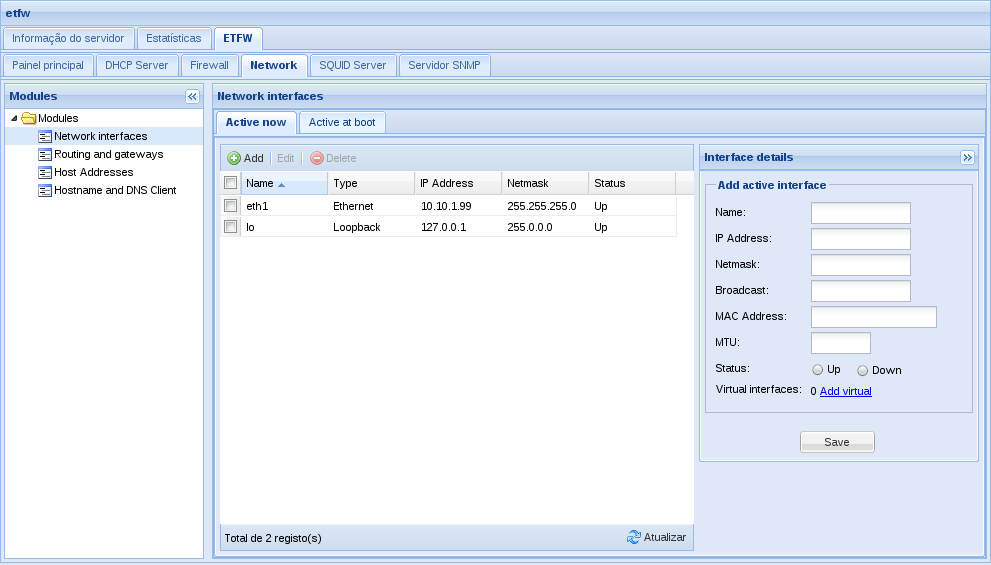
\includegraphics[scale=0.38]{screenshots/etfw/etfw_network_interfaces_01.png}
    \caption{Active interfaces}
    \label{fig:etfw_network_interfaces_01}
    \end{center}
\end{figure}

\begin{figure}[H]
    \begin{center}
    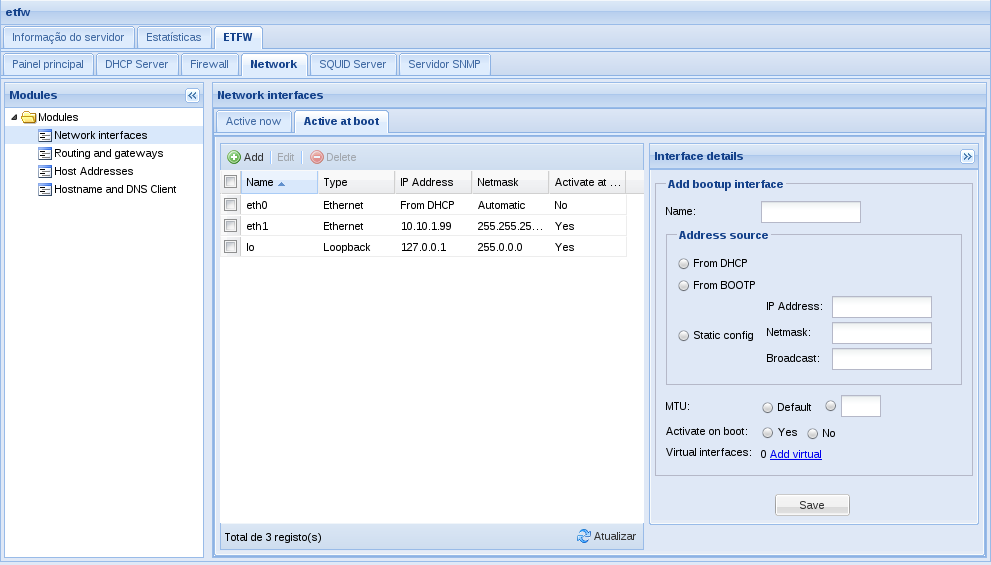
\includegraphics[scale=0.38]{screenshots/etfw/etfw_network_interfaces_02.png}
    \caption{After boot active interfaces}
    \label{fig:etfw_network_interfaces_02}
    \end{center}
\end{figure}

If you wish to define an alias for a network interface, you must select the desired interface, edit and choose \textit{Add virtual} in \textit{Virtual interfaces}. Next, fill out the required parameters and save.

\begin{figure}[H]
    \begin{center}
    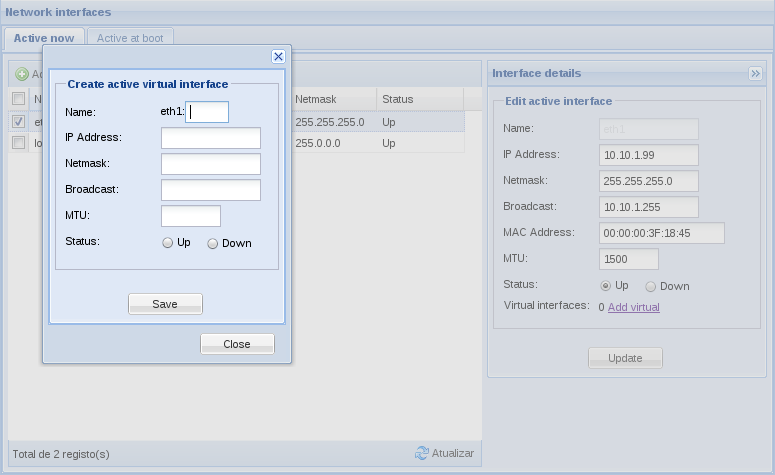
\includegraphics[scale=0.38]{screenshots/etfw/etfw_network_interfaces_03.png}
    \caption{Alias interface}
    \label{fig:etfw_network_interfaces_02}
    \end{center}
\end{figure}

\begin{figure}[H]
    \begin{center}
    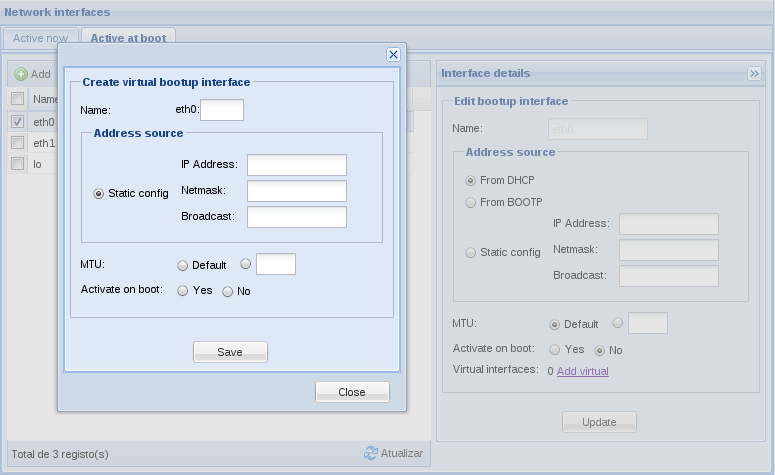
\includegraphics[scale=0.38]{screenshots/etfw/etfw_network_interfaces_04.png}
    \caption{Alias interface active at boot}
    \label{fig:etfw_network_interfaces_02}
    \end{center}
\end{figure}

\subsubsection{Routing and gateways}
In \textit{Routing and gateways} we can query the active routing rules and remove or add new rules.
We can also define routing rules that are set at startup.

\begin{figure}[H]
    \begin{center}
    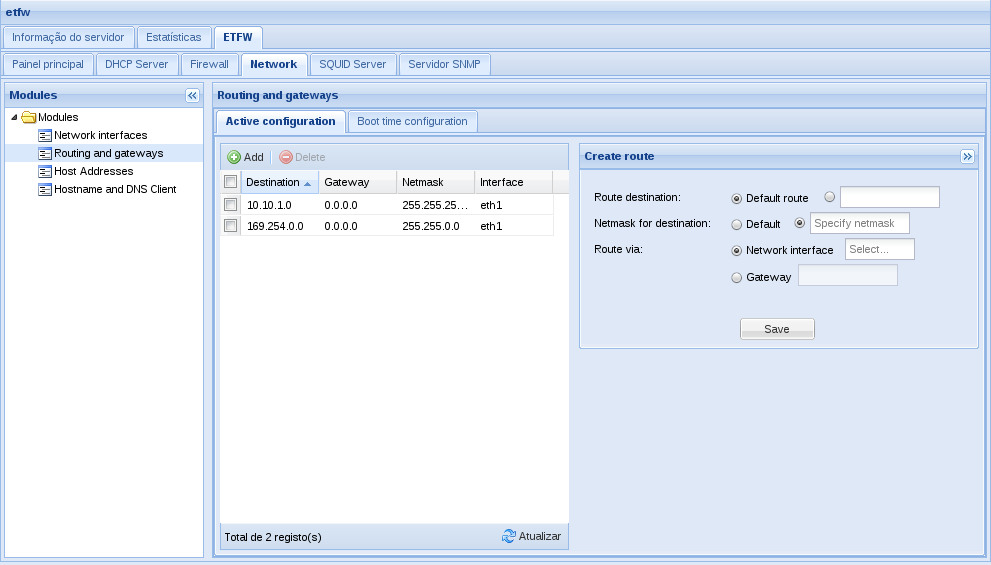
\includegraphics[scale=0.38]{screenshots/etfw/etfw_network_routing_01.png}
    \caption{Active forwarding rules}
    \label{fig:etfw_network_routing_01}
    \end{center}
\end{figure}

To create a routing rule, we choose the \textit{add} option and define the parameters of the route:

\begin{itemize}
    \item \textit{Route destination} - Destination of the forwarding route. It can be \textit{default}, destination IP address or network address;
    \item \textit{Netmask for destination} - Netmask for the route of destination;
    \item \textit{Route via} - \textit{Gateway} or network interface of output route.
\end{itemize}

\begin{figure}[H]
    \begin{center}
    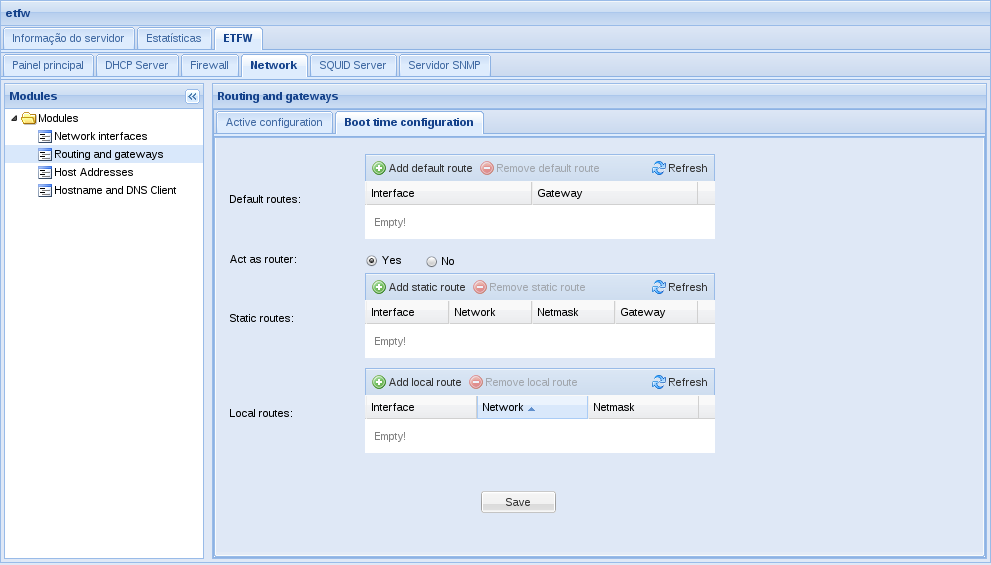
\includegraphics[scale=0.38]{screenshots/etfw/etfw_network_routing_02.png}
    \caption{Defined routing rules at startup}
    \label{fig:etfw_network_routing_02}
    \end{center}
\end{figure}

In the routing rules defined at startup we can configure the following rule types:
\begin{itemize}
    \item \textit{Default routes} - to define the default gateway;
    \item \textit{Static routes} - static routes to other networks/machines;
    \item \textit{Local routes} - static routes where IP addresses are defined, netmask and the interface of each route.
\end{itemize}

\subsubsection{Host Addresses}
In \textit{Host Addresses} you can define static names and locals, associated with IP addresses, in order to reduce response time in name resolution.

\begin{figure}[H]
    \begin{center}
    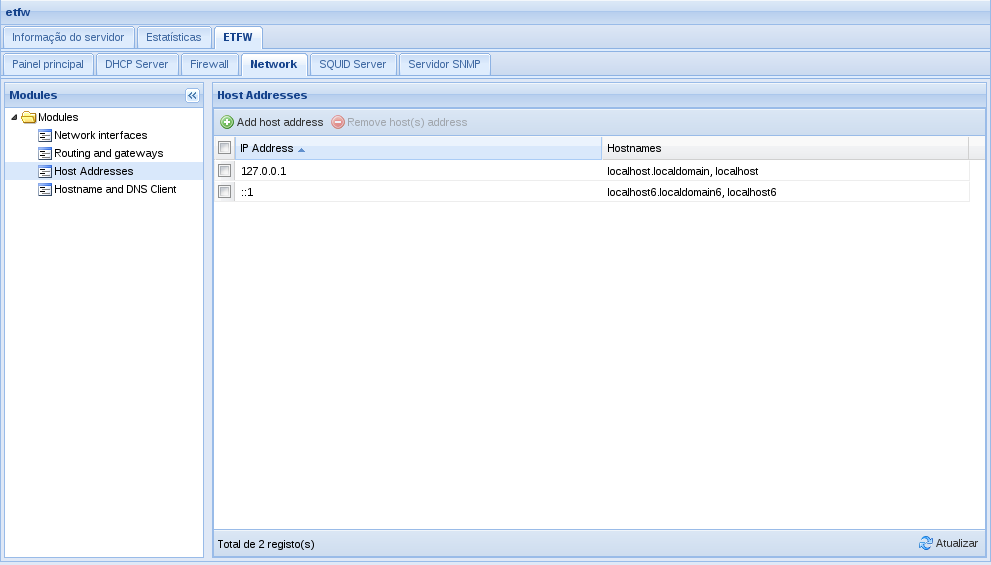
\includegraphics[scale=0.38]{screenshots/etfw/etfw_network_hostaddresses_01.png}
    \caption{Address setup}
    \label{fig:etfw_network_hostaddresses_01}
    \end{center}
\end{figure}

\subsubsection{Hostname and DNS Client}
From this option you can set the name that the machine will have locally and the configuration parameters of the DNS client service (DNS server addresses, order of name resolution on addresses and search domains names).

\begin{figure}[H]
    \begin{center}
    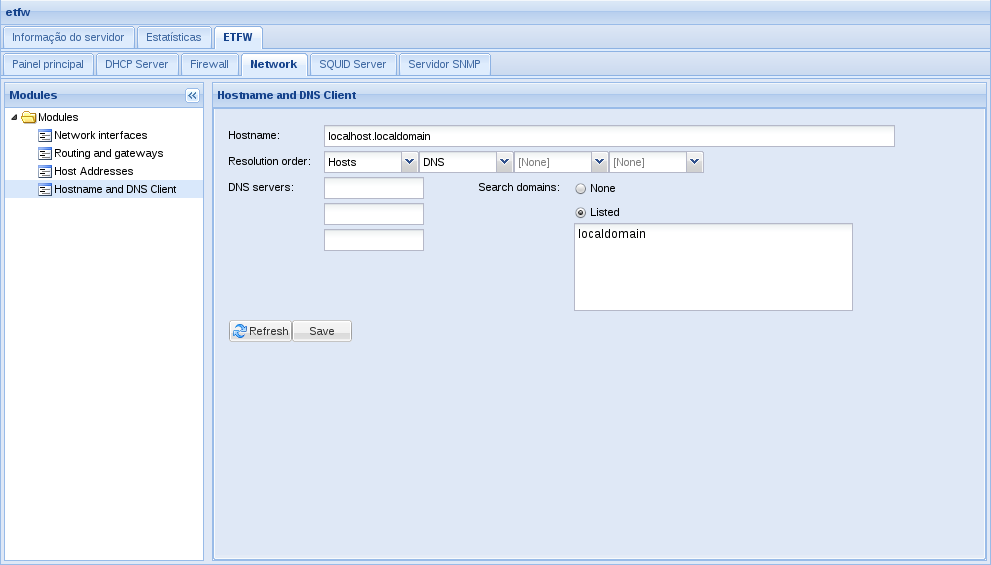
\includegraphics[scale=0.38]{screenshots/etfw/etfw_network_dnsclient_01.png}
    \caption{DNS client}
    \label{fig:etfw_network_dnsclient_01}
    \end{center}
\end{figure}

\subsection{Firewall rules}
By accessing the tab \textit{Firewall} we have the ability to set the rules of Firewall.
This firewall is based on \textit{iptables}, formed by three basic objects:

\begin{itemize}
    \item Rules
    \item Chains
    \item Tables
\end{itemize}

The rules are lower-level objects that perform packet filtering or manipulation.
A rule consists of the following parts:

\begin{itemize}
\item The table were the rule will be added;
\item The chain chain to which the rule will be added;
\item The filtering or manipulation instructions.
\end{itemize}

The rules are organized in chains and act as a checklist of rules ordered.

The chains are organized in tables that group a large number of possible rules to filter and/or manipulate packets.

The operation of the firewall proceeds as follows: if the packet header meet the requirements of the rule, this will follow the destiny imposed by the rule, otherwise it will be evaluated further by the next rule.
%When there are no more rules will be applied the package the default rule or standard set.

\begin{figure}[H]
    \begin{center}
    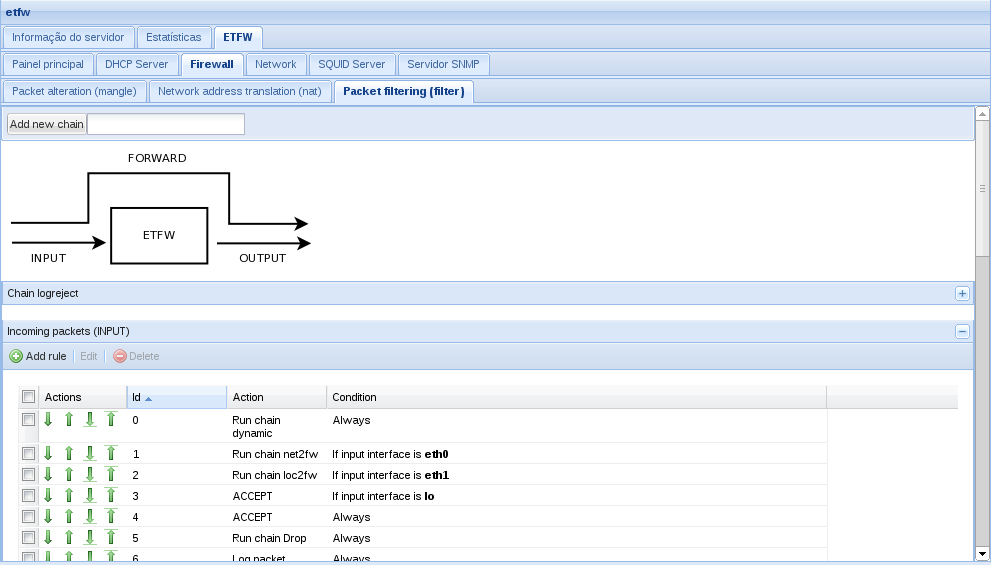
\includegraphics[scale=0.38]{screenshots/etfw/etfw_firewall_01.png}
    \caption{Firewall: Filter table}
    \label{fig:etfw_firewall_01}
    \end{center}
\end{figure}

By accessing the firewall tab the interface shows three tables: \textit{Packet alteration} - \textit{mangle}, \textit{Network address translation} - \textit{nat} and \textit{Packet filtering} - \textit{filter}.

\subsubsection{Table \textit{Filter} - \textit{Packet Filtering}}
The table \textit{filter} is used to filter packets that pass through the firewall and presents three firewall pre-defined chains:

\begin {itemize}
   \item \textbf{INPUT} - filter packets whose destination is the own firewall;
   \item \textbf{OUTPUT} - filters packets whose origin is firewall;
   \item \textbf{FORWARD} - filter packets that pass through the firewall which are not the source nor the destination of the firewall.
\end {itemize}

\begin{figure}[H]
    \begin{center}
    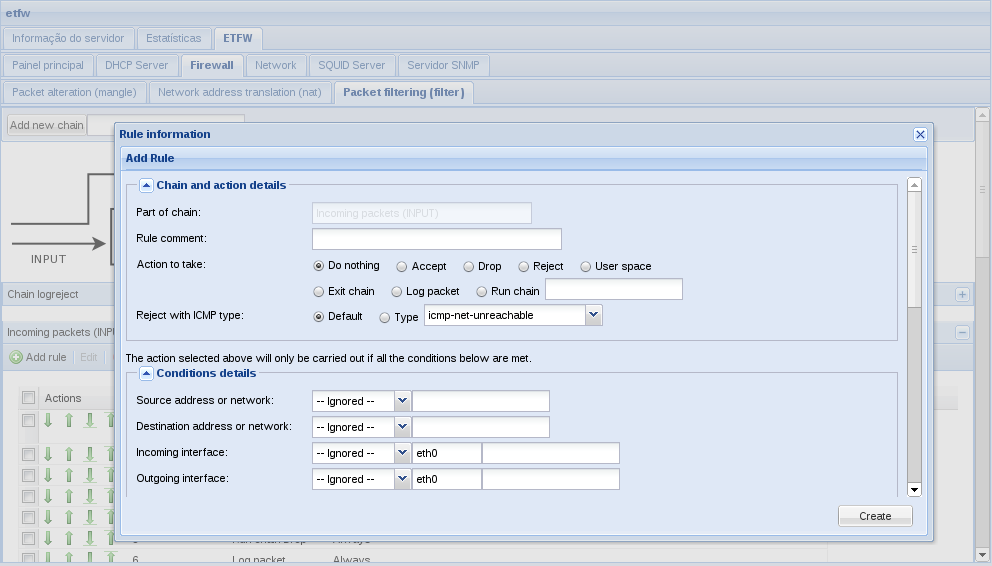
\includegraphics[scale=0.38]{screenshots/etfw/etfw_firewall_02.png}
    \caption{Creating a rule on table \textit{filter} - Chain and action}
    \label{fig:etfw_firewall_02}
    \end{center}
\end{figure}

When creating a rule in a filter table's chain some parameters are required for action to take:

\begin{itemize}
   \item \textbf{Rule comment} - allows you to write a short comment to identify the rule to be created;
   \item \textbf{Action to take} - action to be taken, who decides what should be done with the package, if it matches the rule. The most important actions are:
       \subitem \textbf{Drop} - removes the packet without doing anything else;
       \subitem \textbf{Accept} - the firewall lets the packet pass through and the data is sent to the recipient;
       \subitem \textbf{Reject} - works the same way as the drop but is sent an \textit {ICMP} error back to the sender of the package;
       \subitem \textbf{Userspace} - if this option is active, a multicast is donne by kernel into a socket where can be a listening process.
\end{itemize}

\begin{figure}[H]
    \begin{center}
    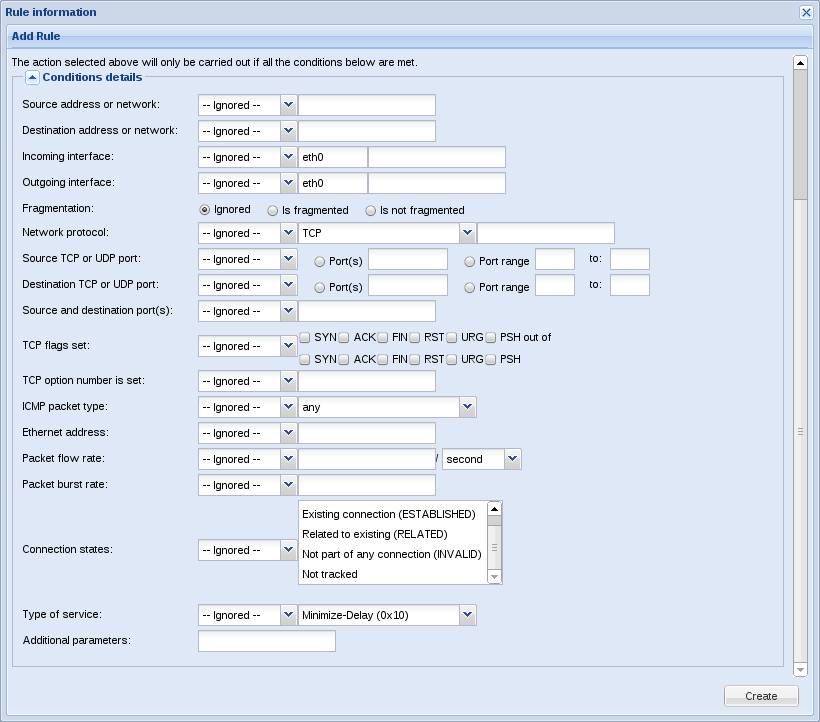
\includegraphics[scale=0.38]{screenshots/etfw/etfw_firewall_03.png}
    \caption{Creating a rule on table \textit{filter} - Condition details}
    \label{fig:etfw_firewall_03}
    \end{center}
\end{figure}

Other options that can be completed in the condition are the following:
\begin{itemize}
    \item \textbf{Source address or network} - Network address that establish the origin of the package. It is usually a combination of IP address with the subnet mask separated by a slash (eg 192.168.1.0/255.255.255.0 or 192.168.1.0/24);
    \item \textbf{Destination address or network} - Network address to which the packet is intended. It has the same combination as before;
    \item \textbf{Incoming interface} - Specifies the input interface of the package;
    \item \textbf{Outgoing interface} - Specifies the output interface of the package;
    \item \textbf{Fragmentation} - Sometimes a packet undergoes fragmentation because of its size, being its part joined together later in the destination. This option sets whether the rule is matched by fragmented packets or not;
    \item \textbf{Network protocol} - Network protocol;
    \item \textbf{Source TCP or UDP port} - Sets the match rule with the incoming port (tcp or udp), and may be defined a range of ports (example: 1000:1050) or a list doors separated by commas;
    \item \textbf{Destination TCP or UDP port} - Sets the output port match and may be offered a range of ports (example: 1000:1050) or a list of ports separated by commas;
    \item \textbf{Source and destination port(s)} - Sets the door match, both incoming and outgoing, may be offered a range of ports or a list of ports separated by commas;
    \item \textbf{ICMP packet type} - ICMP packet type;
    \item \textbf{Ethernet address} - Defines a physical address of a network that will serve to match the rule;
    \item \textbf{Packet flow rate} - Sets the volume of packages that will make the rule match;
    \item \textbf{Packet burst rate} - Sets the threshold at which the packets begin to make match with the rule;
    \item \textbf{Connection states} - Specifies the number of links that make the rule match;
    \item \textbf{Type of service} - Defines the type of service for which we want the rule to do match;
    \item \textbf{Additional parameters} - Specifies additional parameters that will be passed directly to the line of the rule to be applied.
\end{itemize}

\subsubsection{NAT table - Network address translation}
The NAT table is used for network address translation, or translate a package with a particular field of origin or destination.
Only the first packet will be affected by this chain, after which the remaining packages will apply the same actions as the first.
This table presents three pre-defined chains:

\begin{itemize}
    \item \textbf{PREROUTING} - applies the changes to the packages when the target needs to be changed;
    \item \textbf{POSTROUTING} - applies the changes to the packages when the source needs to be changed;
    \item \textbf{OUTPUT} - applies the changes to packets originated by the firewall.
\end{itemize}

The current targets in this table are:

\begin{itemize}
    \item \textbf{DNAT} - used in cases where you have a public IP address in the firewall and if you want to redirect the access to another host (a DMZ for example), thus allowing forward traffic.
    \item \textbf{SNAT} - used when you want to change the origin of package, usually to hide the addresses of local network or \textit{DMZ}.
    \item \textbf{MASQUERADE} - used the same way that the SNAT and for the same reason, but the outgoing IP address is not specified, by using the source address of the interface package. This rule is used primarily for dynamic IP addresses, because if the link goes down, the source address that was being used is discarded yielding place to a new source address of the interface when the connection is restored.
\end{itemize}

\begin{figure}[H]
    \begin{center}
    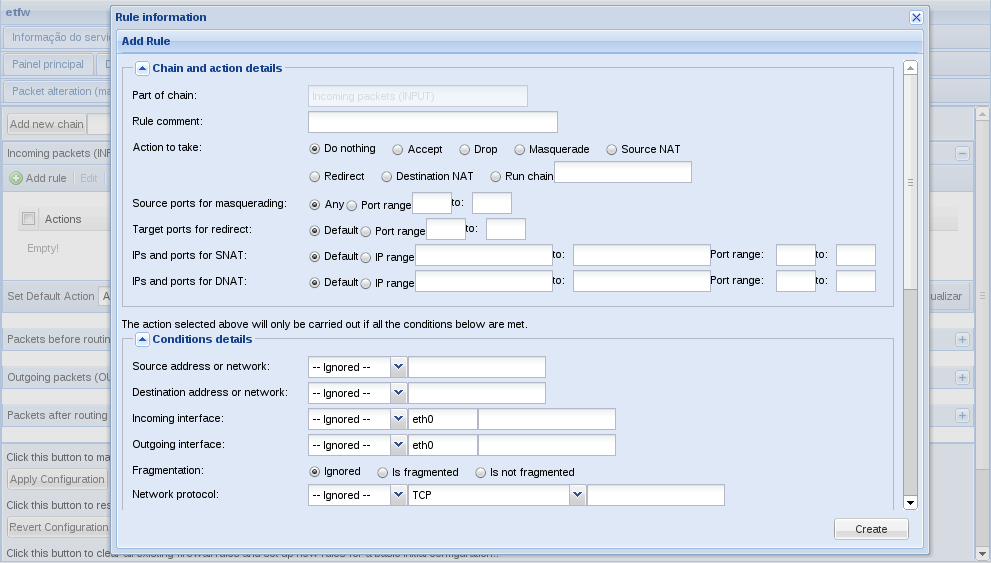
\includegraphics[scale=0.38]{screenshots/etfw/etfw_firewall_04.png}
    \caption{Creating a rule on NAT table}
    \label{fig:etfw_firewall_03}
    \end{center}
\end{figure}

The options used in the NAT table are identical to the Filter table. The differences are listed bellow:

\begin{itemize}
    \item \textbf{Action to take} - action to be taken, has the same functionality described in the Filter table, but has two different options:
        \subitem \textbf{Masquerade} - Rewrites the outgoing IP address, when it comes to dynamic IP addresses;
        \subitem \textbf{Source NAT} / \textbf{Destination NAT} - Depending on the chain (PREROUTING, POSTROUTING or OUTPUT), available options may vary. They will be \textit{Source NAT} and \textit{estination NAT}, respectively. Also, they will re-write the IP's input and output respectively.
\end{itemize}

\subsubsection{Mangle table - Packet alteration}

This table is not addressed in this version of the manual.

\subsection{DHCP Server}
In this tab we can configure the DHCP server, including IP range to allocate the hosts, router address, DNS server address, view active leases, and to start/stop the server.

\begin{figure}[H]
    \begin{center}
    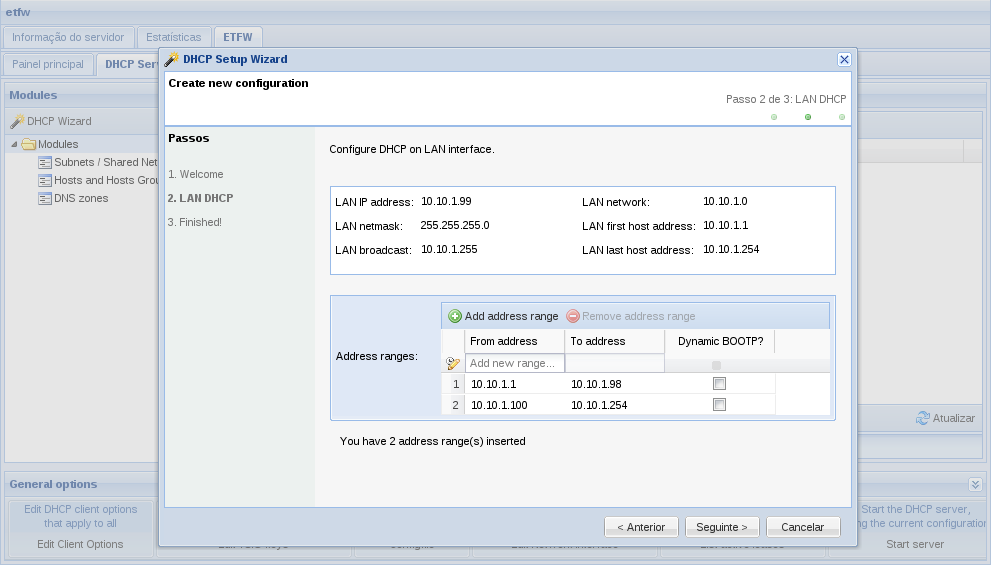
\includegraphics[scale=0.38]{screenshots/etfw/etfw_dhcp_wizard_01.png}
    \caption{IP range setup}
    \label{fig:etfw_dhcp_wizard_01}
    \end{center}
\end{figure}

From the DHCP Wizard we can, in a first stage, set the IP ranges allocated to hosts.

\begin{figure}[H]
    \begin{center}
    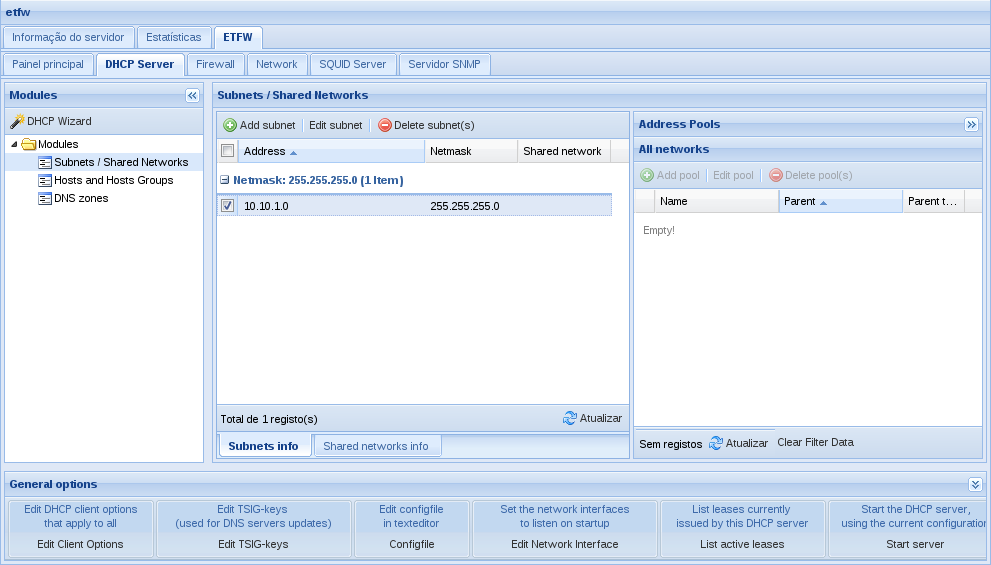
\includegraphics[scale=0.38]{screenshots/etfw/etfw_dhcp_subnets_01.png}
    \caption{Subnets setup}
    \label{fig:etfw_dhcp_subnets_01}
    \end{center}
\end{figure}

\begin{figure}[H]
    \begin{center}
    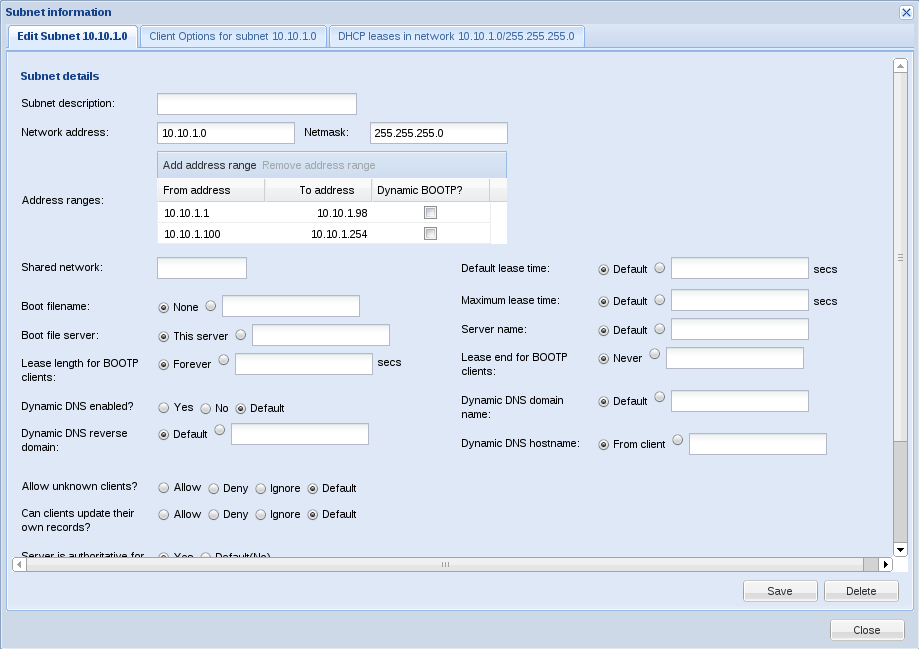
\includegraphics[scale=0.38]{screenshots/etfw/etfw_dhcp_subnets_02.png}
    \caption{Subnet edit}
    \label{fig:etfw_dhcp_subnets_02}
    \end{center}
\end{figure}

Later, you can edit the subnets and set the appropriate parameters to our setting for the network address, netmask, address range, among others.

\begin{figure}[H]
    \begin{center}
    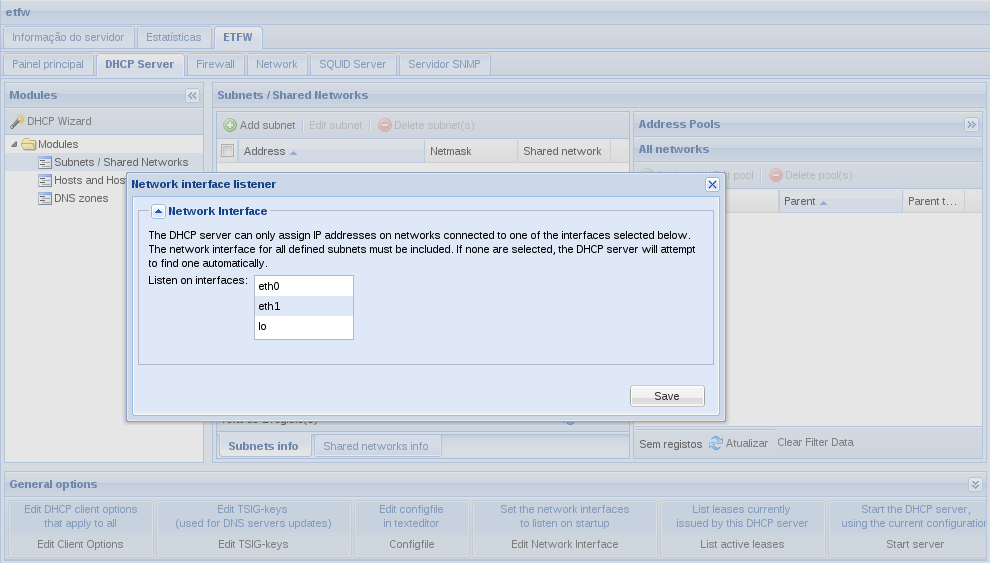
\includegraphics[scale=0.38]{screenshots/etfw/etfw_dhcp_interfaces_01.png}
    \caption{Choose an interface}
    \label{fig:etfw_dhcp_interfaces_01}
    \end{center}
\end{figure}

To configure the server properly you must set the interface on which service will operate.
Go to \textit{Edit Network Interface} and choose the desired network interface.

\begin{figure}[H]
    \begin{center}
    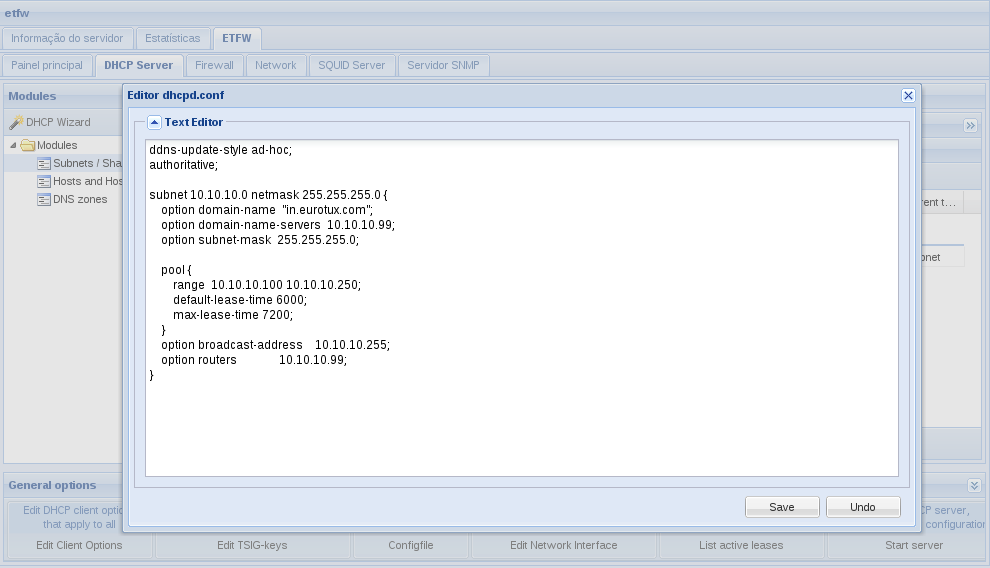
\includegraphics[scale=0.38]{screenshots/etfw/etfw_dhcp_texteditor_01.png}
    \caption{Configuration file edition}
    \label{fig:etfw_dhcp_texteditor_01}
    \end{center}
\end{figure}

Additionally, you can always view and edit the configuration file directly and put the desired options.

\begin{figure}[H]
    \begin{center}
    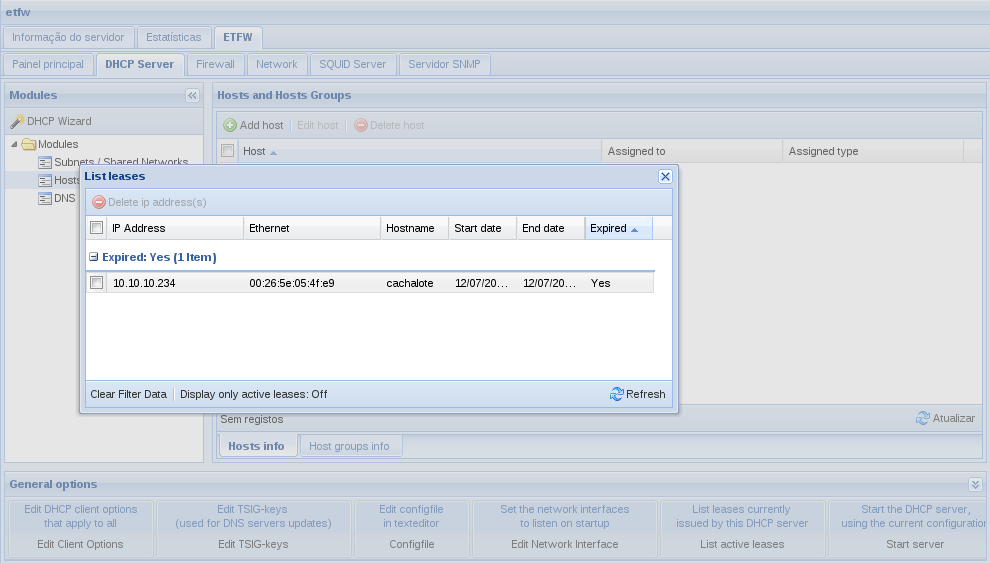
\includegraphics[scale=0.38]{screenshots/etfw/etfw_dhcp_leases_01.png}
    \caption{List of active leases}
    \label{fig:etfw_dhcp_leases_01}
    \end{center}
\end{figure}

In any time you can find a list of assigned IPs by selecting the option \textit{List active leases}. This option is also available for each subnet.

\subsection{SQUID server}

In the \textit{SQUID Server} tab you can configure the SQUID Proxy service.

\begin{figure}[H]
    \begin{center}
    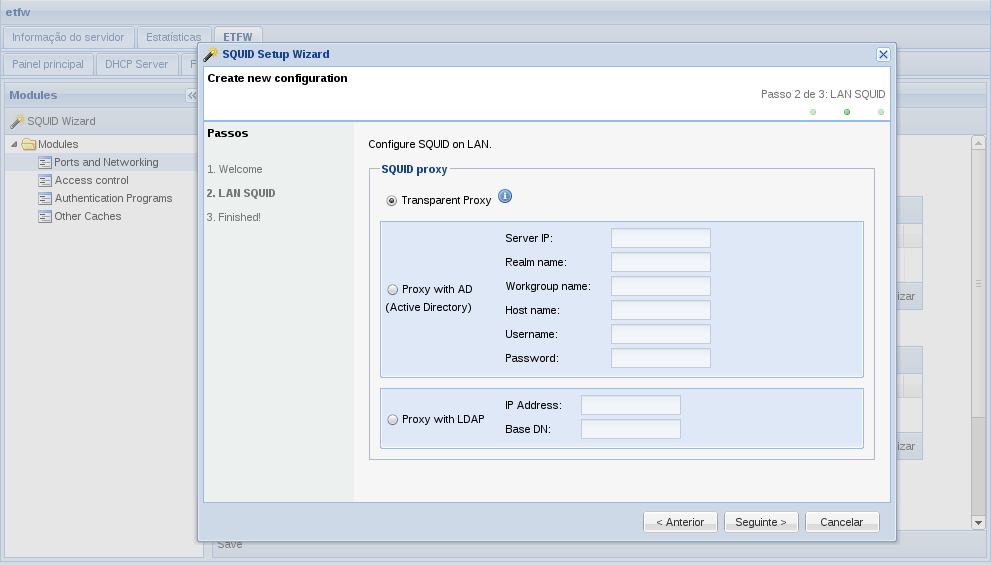
\includegraphics[scale=0.38]{screenshots/etfw/etfw_squid_wizard_01.png}
    \caption{SQUID server setup}
    \label{fig:etfw_squid_wizard_01}
    \end{center}
\end{figure}

The proxy service forward requests to the Internet and keeps a content's cache in a way to speed up the display when they are requested again.

In the \textit{SQUID Wizard} we can configure the proxy service easily. It has three pre-defined configuration options:

\begin{itemize}
    \item \textit{Transparent Proxy} - Transparent Proxy;
    \item \textit{Proxy with AD} - Proxy with authentication in Active Directory;
    \item \textit{Proxy with LDAP} - Proxy with LDAP authentication.
\end{itemize}

In the first case, the transparent proxy, allows you to have a cache system cache completely invisible to the customers. This system does not support authentication.

In the other two cases, the proxy makes use of authentication systems, such as Active Directory or LDAP.

Additionally, you can customize the service in accordance with the needs, in particular define: Ports and Networking, Access Control, Authentication Programs, among other types of cache.

\subsubsection{Ports and Networking}

In \textit{Ports and Networking} you can define the port (SSL or not), and IP address or hostname of the proxy service that will fill orders, in addition to other possible configurations, including:

\begin{figure}[H]
    \begin{center}
    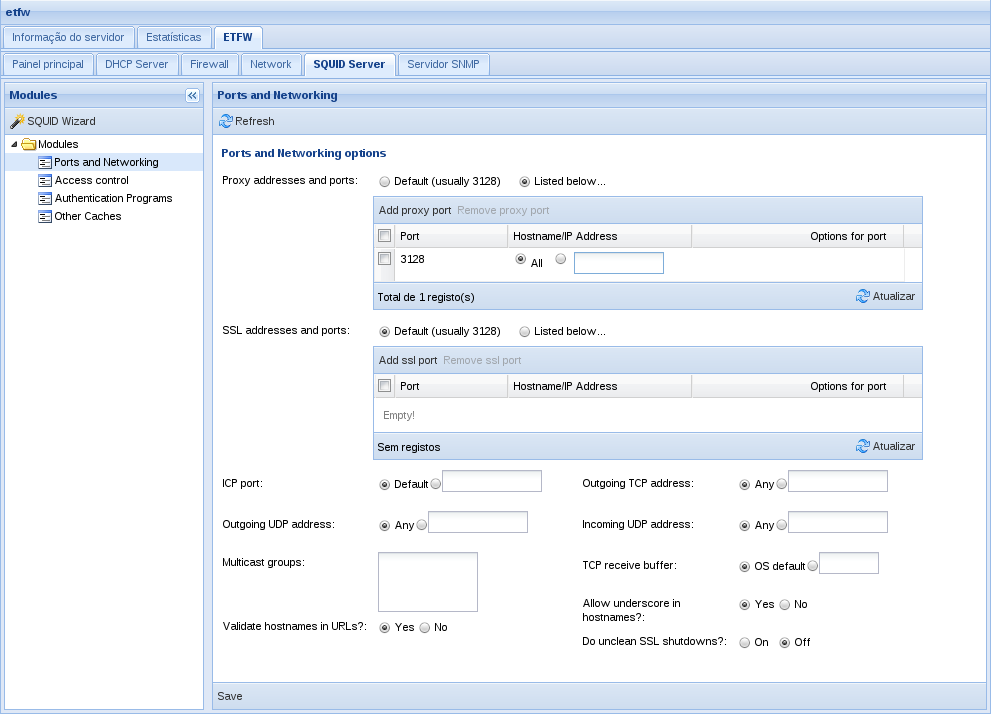
\includegraphics[scale=0.38]{screenshots/etfw/etfw_squid_portsnetworking_01.png}
    \caption{Port and network configuration}
    \label{fig:etfw_squid_portsnetworking_01}
    \end{center}
\end{figure}

Request port \textit{ICP};
Validation name addresses of URLs;
Specification group \textit{multicast};
Output address of TCP traffic;
Output address UDP traffic;


\begin{itemize}
    \item \textit{ICP port} - ICP request port;
    \item \textit{Validate hostnames in URLs?} - Validation of urls' address;
    \item \textit{Multicast groups} - Multicast groups;
    \item \textit{Outgoing TCP address} - Output address for TCP traffic;
    \item \textit{Outgoing UDP address} - Output address for UDP traffic;
    \item \textit{Incoming UDP address} - Input address for UDP traffic;
    \item \textit{TCP receive buffer} - Buffer \textit{TCP};
\end{itemize}

\subsubsection{Access Control}

The access control policies are based on a combination of \textit{ACL}(\textit{Access Control Lists}).

\begin{figure}[H]
    \begin{center}
    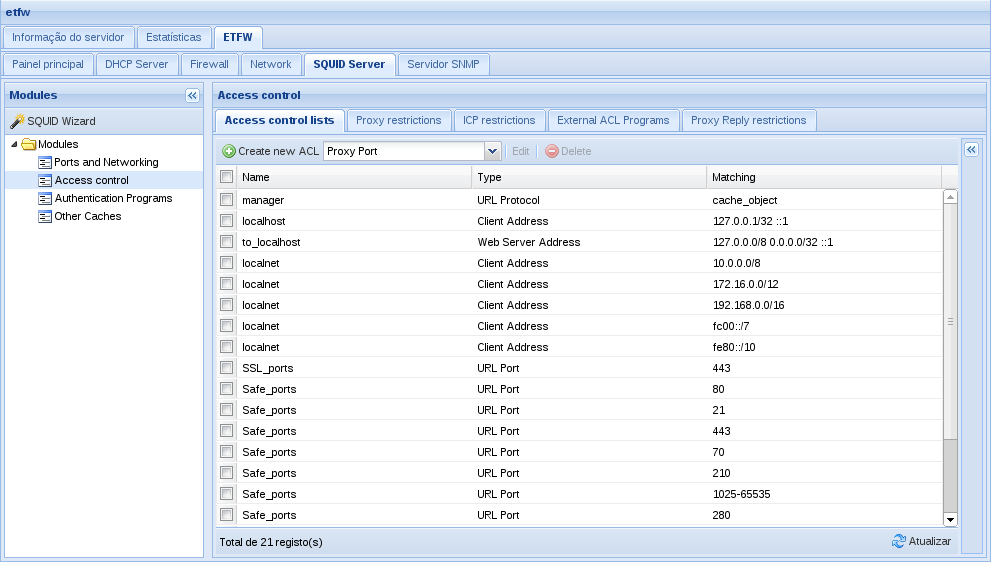
\includegraphics[scale=0.38]{screenshots/etfw/etfw_squid_accesscontrol_01.png}
    \caption{Setup of access control policies}
    \label{fig:etfw_squid_accesscontrol_01}
    \end{center}
\end{figure}

In the configuration of access control policies we can define filtering models that can be used later in the sections of restrictions of access (\textit{Proxy Restrictions}, \textit{ICP Restrictions}, \textit{Proxy Reply Restrictions}) .

\begin{figure}[H]
    \begin{center}
    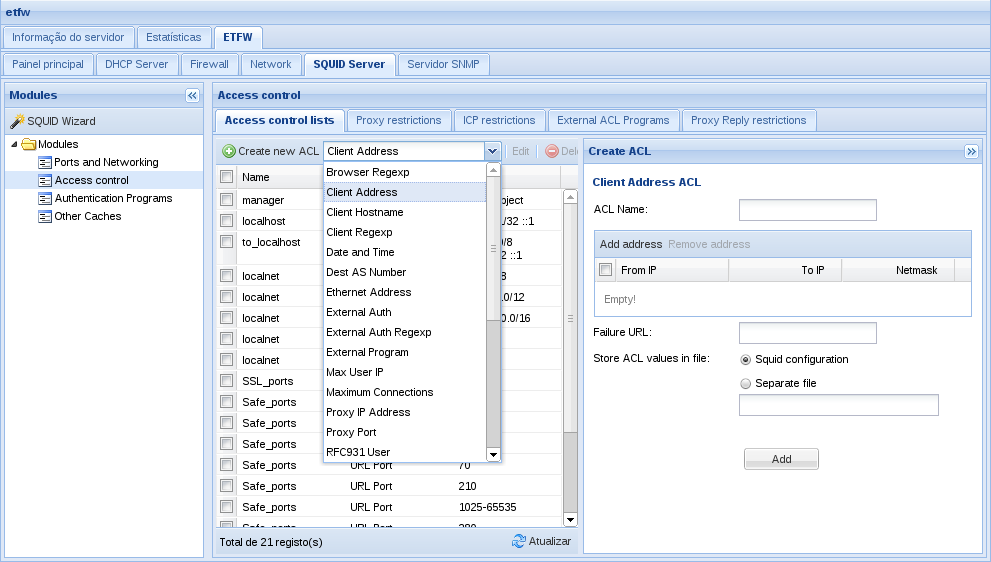
\includegraphics[scale=0.38]{screenshots/etfw/etfw_squid_accesscontrol_02.png}
    \caption{Creating a new ACL}
    \label{fig:etfw_squid_accesscontrol_02}
    \end{center}
\end{figure}

To create a new ACL, we select the type and fill with the desired parameters.

\begin{figure}[H]
    \begin{center}
    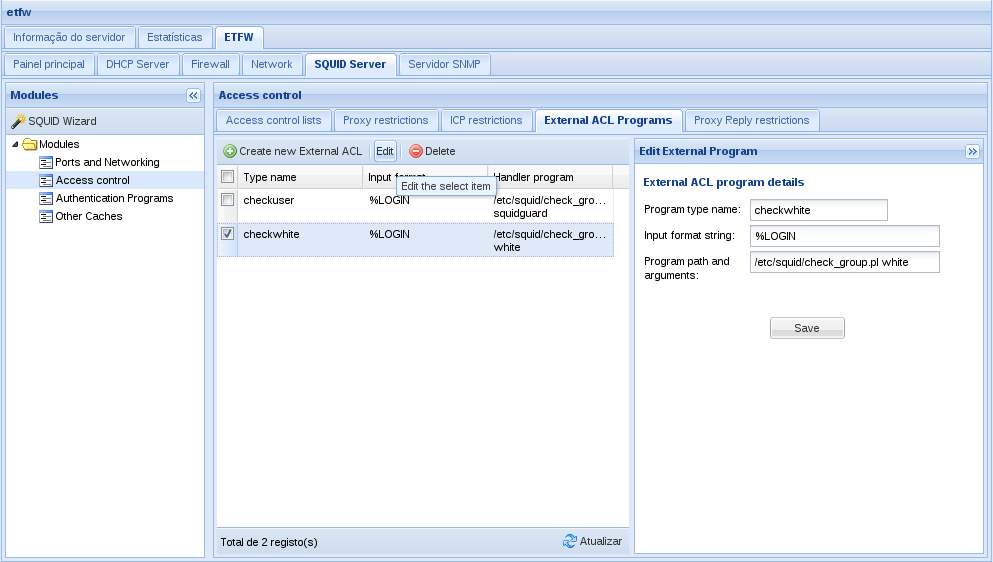
\includegraphics[scale=0.38]{screenshots/etfw/etfw_squid_accesscontrol_03.png}
    \caption{Creating a new external acl}
    \label{fig:etfw_squid_accesscontrol_03}
    \end{center}
\end{figure}

It is also possible to define external ACLs that allow to expand the functionalities of the proxy, using for this purpose external programs that manage the access.
These ACLs allow, for example, the authentication in a server such as a Active Directory or a LDAP, or even the verification of source addresses in a SQL database.

The creation of an external \textit{ACL} external requires the creation of an internal ACL with reference to the first one.

\begin{figure}[H]
    \begin{center}
    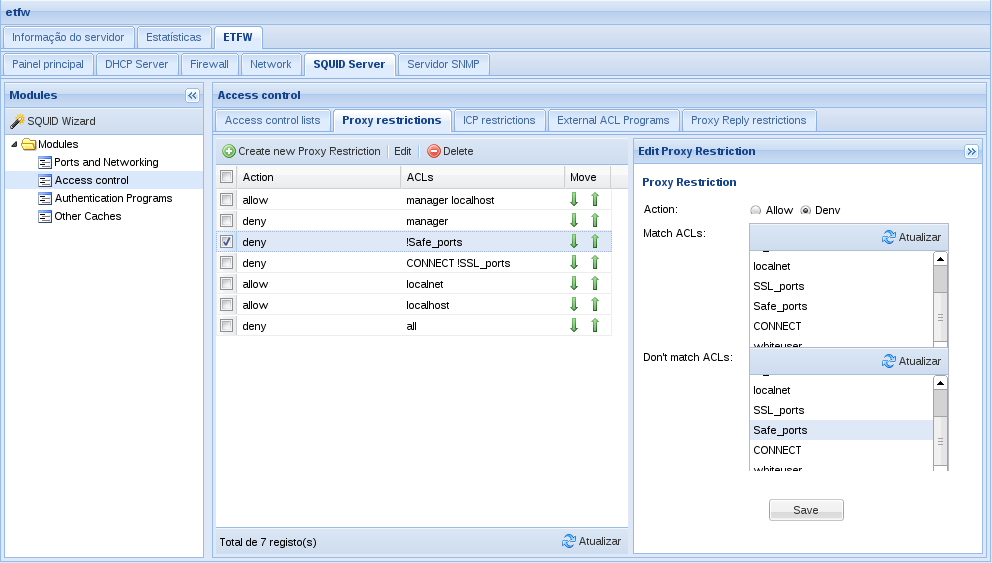
\includegraphics[scale=0.38]{screenshots/etfw/etfw_squid_accesscontrol_04.png}
    \caption{Restriction definition - \textit{Proxy restrictions}}
    \label{fig:etfw_squid_accesscontrol_04}
    \end{center}
\end{figure}

After the ACL definition, you must associate the restrictions with the ACLs to be applied in every situation, or what action to do: accept or deny.
The rules are applied in top-bottom order, and when a match is found the action takes place.
Importantly, if there is a deny all rule, all requests that pass the rules are accepted.

\subsubsection{Authentication Programs}

In \textit{Authentication Programs} are defined programs that ask the browser/user what's his authentication credentials.

\begin{figure}[H]
    \begin{center}
    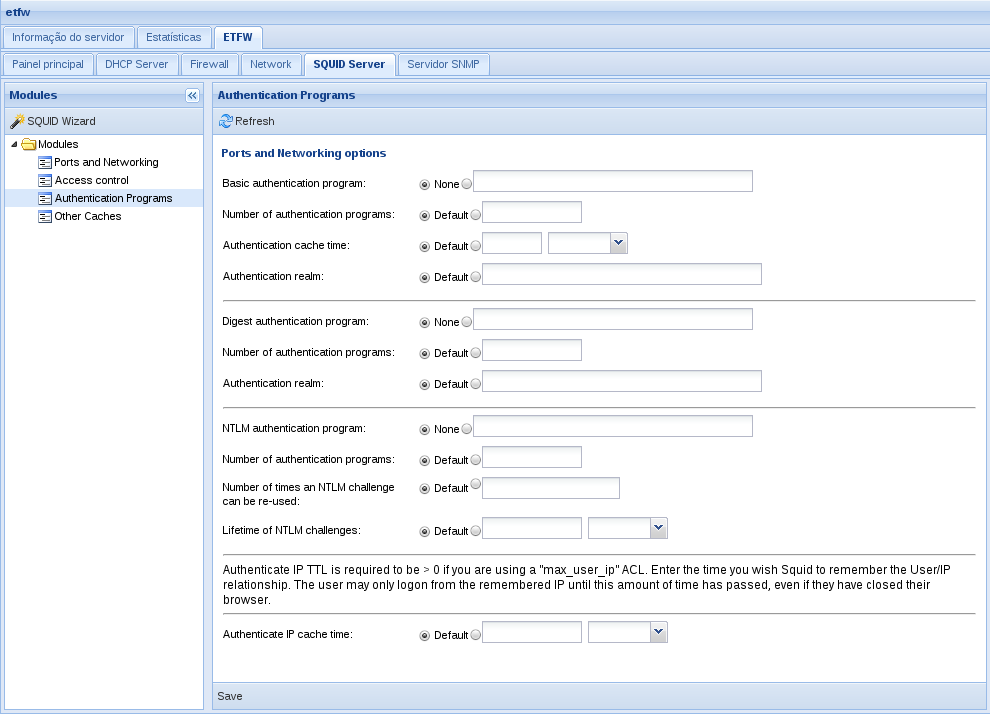
\includegraphics[scale=0.38]{screenshots/etfw/etfw_squid_authenticationprograms_01.png}
    \caption{Authentication Programs}
    \label{fig:etfw_squid_authenticationprograms_01}
    \end{center}
\end{figure}

There are two types of authentication:

\begin{itemize}
    \item \textit{Basic} - when the browser does not support transparent authentication, it will show a popup asking the user credentials
    \item \textit{NTLMSSP} - transparent authentication for the user
\end{itemize}

We can even set the following parameters:

\begin{itemize}
    \item \textit{authentication program} - Specifies the user program for authentication. The program reads a line containing user and the password separated by space, and responds \textit{OK} on success or \textit{ERR} on failure;
    \item \textit{Number of authentication programs} - Maximum number of process that the authentication could have;
    \item \textit{Authentication realm} - Text that will appear in the dialog box in case of basic authentication;
    \item \textit{Authentication cache time} - Specifies how long a valid authentication is maintained avoiding requests;
    \item \textit{Number of times an NTLM challenge can be re-used} - A maximum number of times that can be used in NTLMSSP authentication type;
    \item \textit{Lifetime of NTLM challenges} - Lifetime of the \textit{NTLMSSP} authentication type;
    \item \textit{Authenticate IP cache time} - Specifies for how long the cache is kept about the user-IP association. 
\end{itemize}

\subsubsection{Other Caches}

In \textit{Other caches} we can specify other proxies to be used in a chain the get information.

\begin{figure}[H]
    \begin{center}
    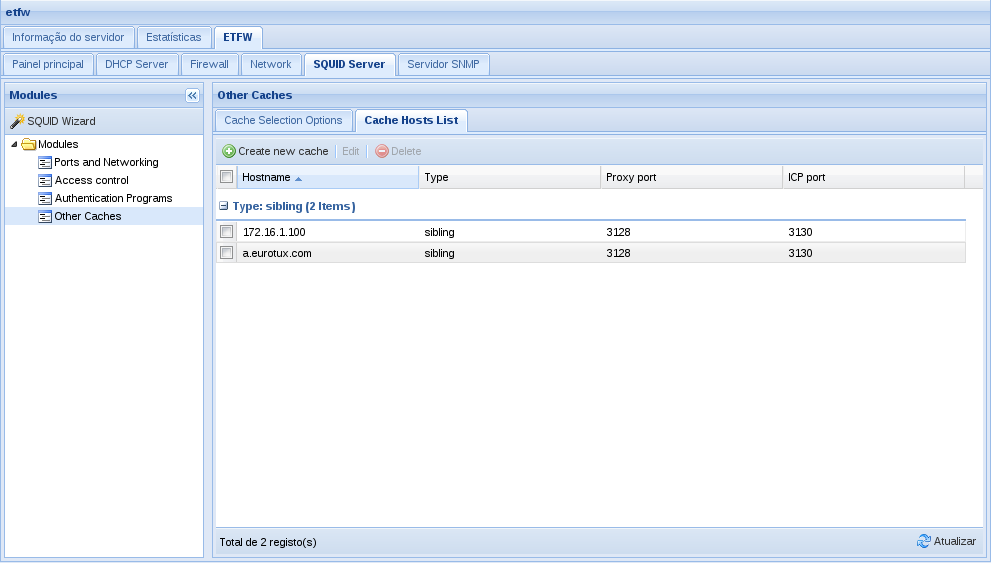
\includegraphics[scale=0.38]{screenshots/etfw/etfw_squid_othercaches_01.png}
    \caption{Proxies - Other Caches}
    \label{fig:etfw_squid_othercaches_01}
    \end{center}
\end{figure}

\begin{figure}[H]
    \begin{center}
    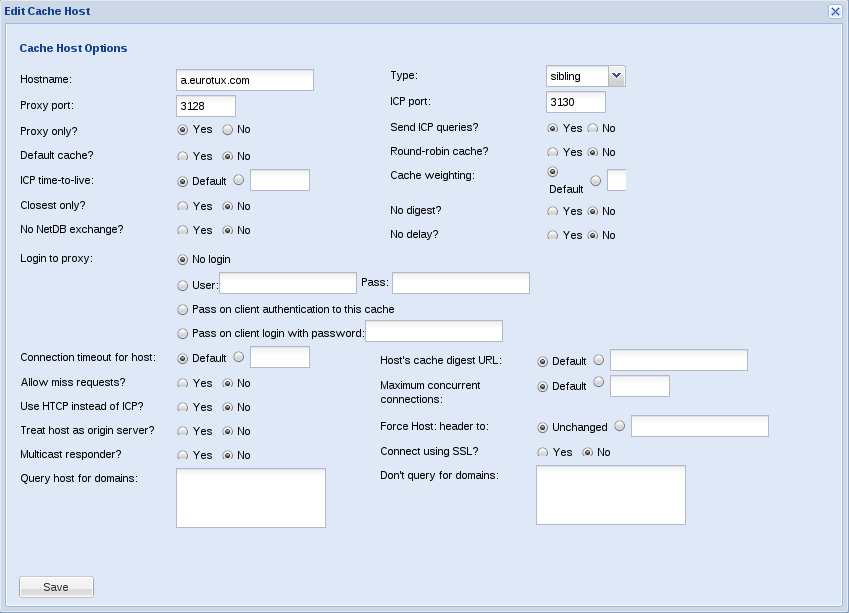
\includegraphics[scale=0.38]{screenshots/etfw/etfw_squid_othercaches_02.png}
    \caption{Edit host cache}
    \label{fig:etfw_squid_othercaches_01}
    \end{center}
\end{figure}

To specify a different proxy it's necessary to specify the following fields:

\begin{itemize}
    \item \textit{Hostname} - IP address or hostname (\textit{FQDN}) of the cache to being used;
    \item \textit{Type} - Type hierarchy to be used between the proxies:
        \subitem \textit{parent};
        \subitem \textit{sibling};
        \subitem \textit{multicast};
    \item \textit{Proxy port} - The port that proxy uses for listening requests;
    \item \textit{ICP port} - Used port to ask neighbors about the cache objects that they have;
    \item \textit{Proxy only?} - Indicates that the requested content to this proxy is not to save locally; 
    \item \textit{Send ICP queries} - Used for proxies that does not have ICP, i.e., that indicates if they have a object or not;
    \item \textit{Default cache} - It is used when the proxy is the last in the hierarchy line;
    \item \textit{Round-robin cache} - To use the round-robin algorithm of search for proxies;
    \item \textit{ICP time-to-live} - Specifies the Time-To-Live(ttl) used in multicast protocol;
    \item \textit{Cache weighting} - Specifies the importance of the cache on the process o choosing proxy (1 for lower priority).
\end{itemize}

\subsubsection{Usage exemples}

\begin{figure}[H]
    \begin{center}
    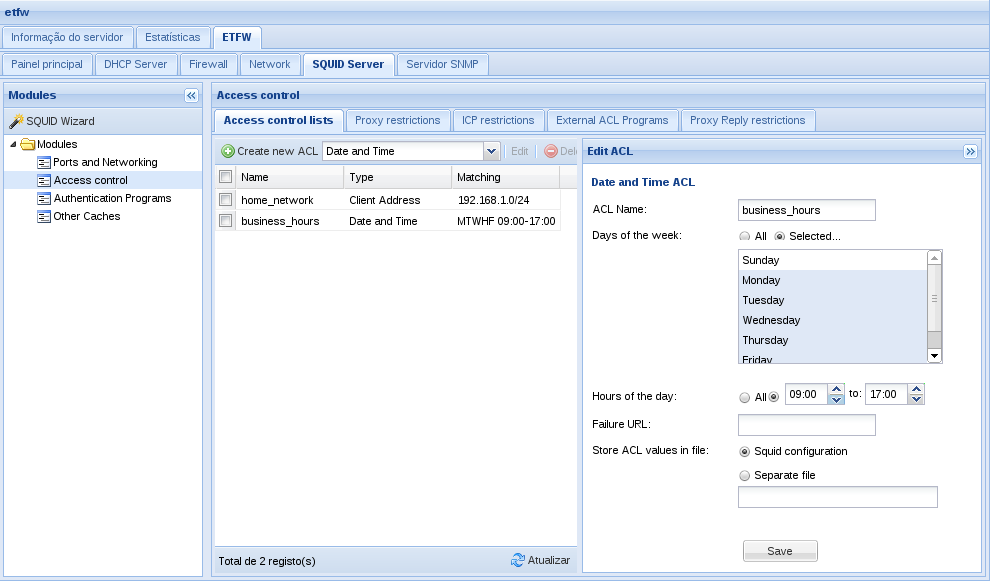
\includegraphics[scale=0.38]{screenshots/etfw/etfw_squid_example_time_01_01.png}
    \caption{Restrict internal network access only during work hours - Creating ACLs.}
    \label{fig:etfw_squid_example_time_01_01}
    \end{center}
\end{figure}

\begin{figure}[H]
    \begin{center}
    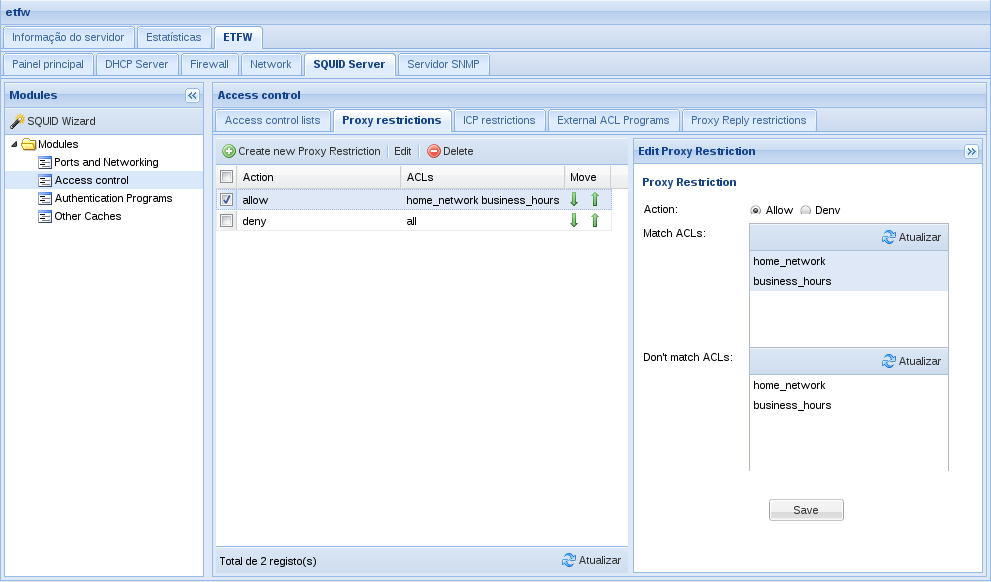
\includegraphics[scale=0.38]{screenshots/etfw/etfw_squid_example_time_01_02.png}
    \caption{Restrict internal network access only during work hours - Creating restriction using previously defined ACLs}
    \label{fig:etfw_squid_example_time_01_02}
    \end{center}
\end{figure}

\begin{figure}[H]
    \begin{center}
    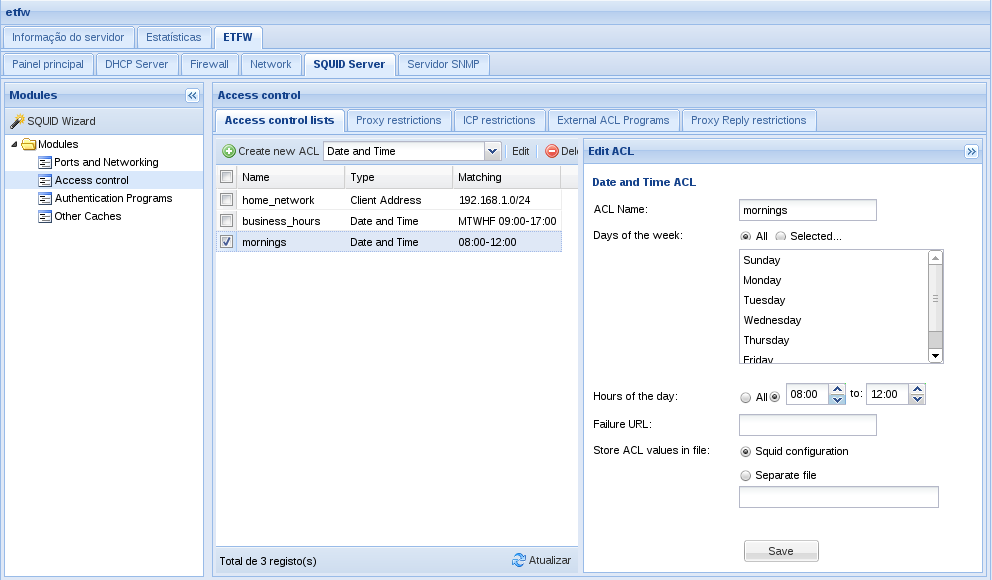
\includegraphics[scale=0.38]{screenshots/etfw/etfw_squid_example_time_02_01.png}
    \caption{Restrict access only in the morning - Creating ACLs}
    \label{fig:etfw_squid_example_time_02_01}
    \end{center}
\end{figure}

\begin{figure}[H]
    \begin{center}
    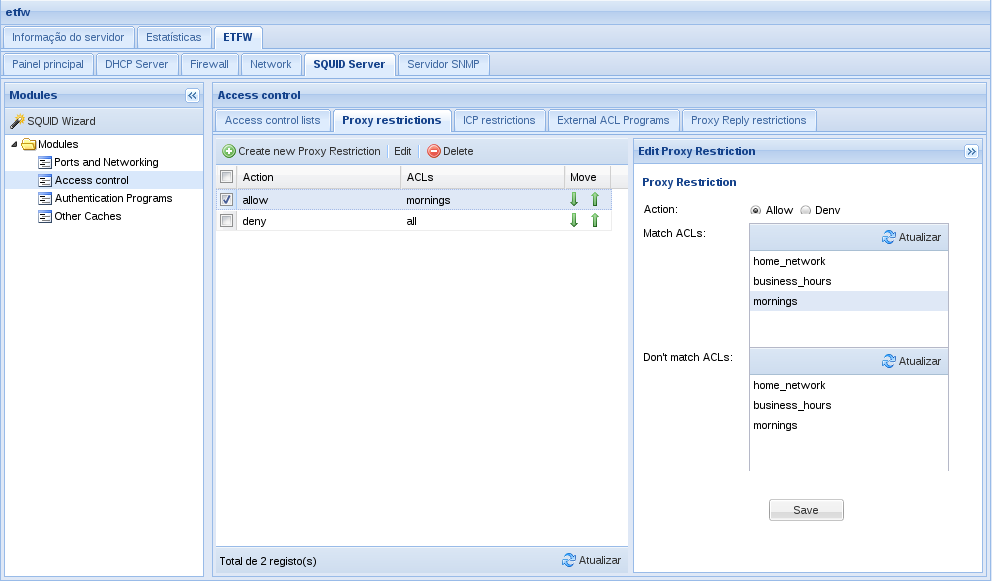
\includegraphics[scale=0.38]{screenshots/etfw/etfw_squid_example_time_02_02.png}
    \caption{Restrict access only in the morning - Creating restriction using previously defined ACLs}
    \label{fig:etfw_squid_example_time_02_02}
    \end{center}
\end{figure}

\begin{figure}[H]
    \begin{center}
    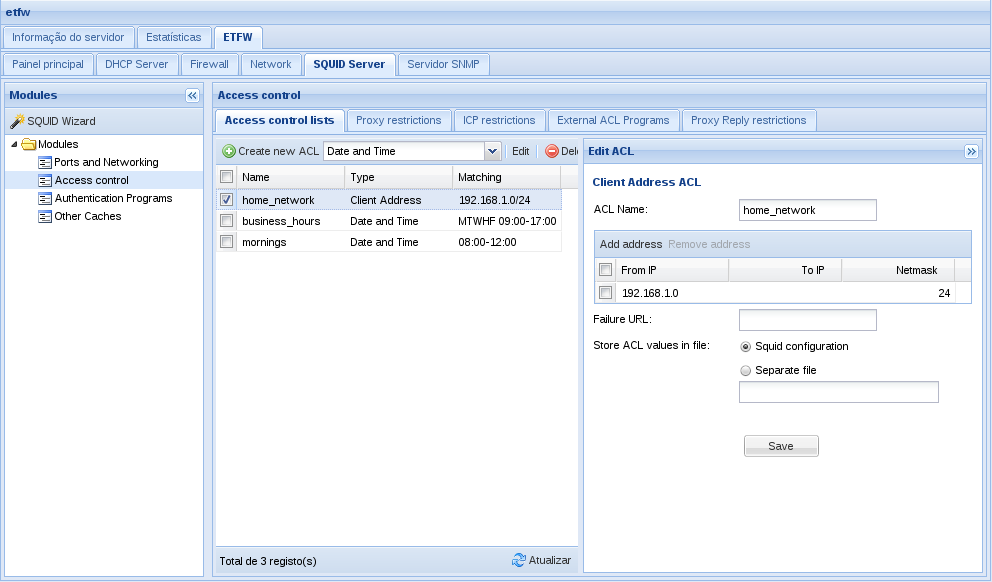
\includegraphics[scale=0.38]{screenshots/etfw/etfw_squid_example_acessoip_01.png}
    \caption{Restrict access by IP address - Creating ACLs}
    \label{fig:etfw_squid_example_acessoip_01}
    \end{center}
\end{figure}

\begin{figure}[H]
    \begin{center}
    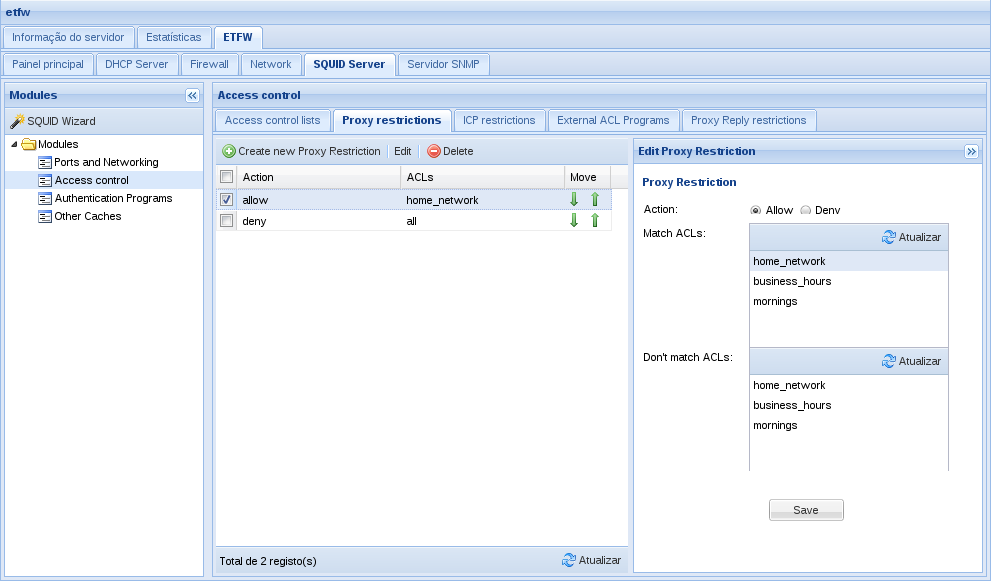
\includegraphics[scale=0.38]{screenshots/etfw/etfw_squid_example_acessoip_02.png}
    \caption{Restrict access by IP address - Creating restriction using previously defined ACLs}
    \label{fig:etfw_squid_example_acessoip_02}
    \end{center}
\end{figure}

\begin{figure}[H]
    \begin{center}
    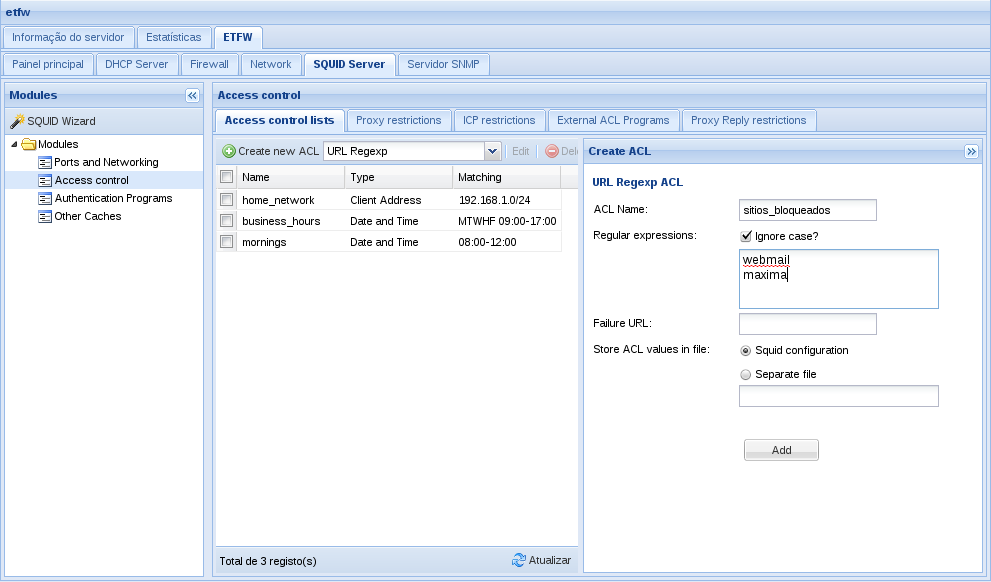
\includegraphics[scale=0.38]{screenshots/etfw/etfw_squid_example_urlregexp_01.png}
    \caption{Denying access based on a regular expression on the URL - Creating ACLs}
    \label{fig:etfw_squid_example_urlregexp_01}
    \end{center}
\end{figure}

\begin{figure}[H]
    \begin{center}
    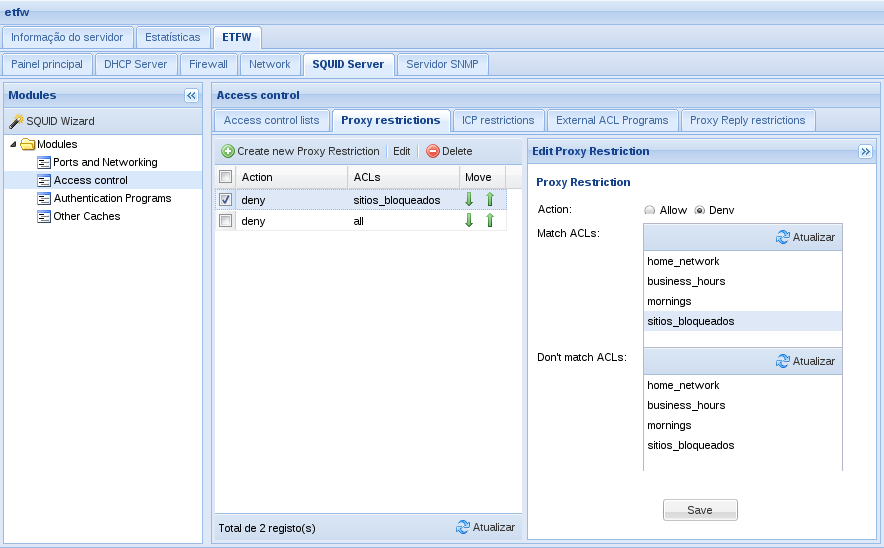
\includegraphics[scale=0.38]{screenshots/etfw/etfw_squid_example_urlregexp_02.png}
    \caption{Denying access based on a regular expression on the URL - Creating restriction using previously defined ACLs}
    \label{fig:etfw_squid_example_urlregexp_02}
    \end{center}
\end{figure}

\subsection{SNMP server}

In the SNMP server configuration interface you can define the following configuration:

\begin{itemize}
    \item System information: location and contact;
    \item Trap server's IP address;
    \item Trap community;
    \item Monitoring stations.
\end{itemize}

\begin{figure}[H]
    \begin{center}
    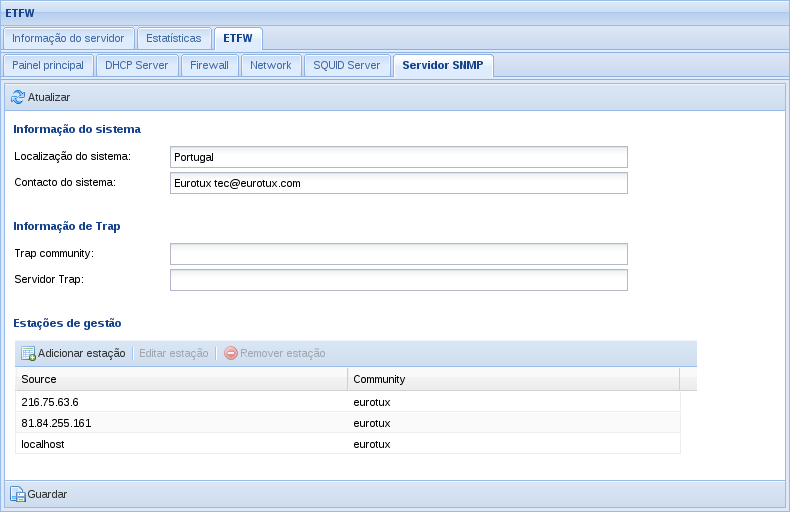
\includegraphics[scale=0.38]{screenshots/etfw/etfw_snmp_01.png}
    \caption{SNMP server setup}
    \label{fig:etfw_smp_01}
    \end{center}
\end{figure}

